\documentclass[11pt,a4paper]{article}

\usepackage[utf8]{inputenc}
\usepackage[T1]{fontenc}
\usepackage[margin=0.85in]{geometry}
\usepackage{amsmath,amsfonts,amssymb}
\usepackage{booktabs}
\usepackage{tabularx}
\usepackage{array}
\usepackage{graphicx}
\usepackage[export]{adjustbox}
\usepackage{hyperref}
\usepackage{xcolor}
\usepackage{enumitem}
\usepackage{titlesec}
\usepackage{fancyhdr}

% Palette matching Aura UI's calm dark accent hierarchy (adapted for white paper)
\definecolor{AuraTeal}{HTML}{2B6B5B}
\definecolor{AuraAmber}{HTML}{A66B1E}
\definecolor{AuraRose}{HTML}{9E3B3B}
\definecolor{AuraSlate}{HTML}{4A4458}
\definecolor{CodeBg}{HTML}{F5F4F8}
\definecolor{CalloutBg}{HTML}{EEF6F3}

\hypersetup{
    colorlinks=true,
    linkcolor=AuraTeal,
    citecolor=AuraTeal,
    urlcolor=blue!65!black
}

\titleformat{\section}{\large\bfseries\color{AuraTeal}}{\thesection}{0.9em}{}[\titlerule]
\titleformat{\subsection}{\normalsize\bfseries\color{AuraSlate}}{\thesubsection}{0.8em}{}

\pagestyle{fancy}
\fancyhf{}
\lhead{\small \textbf{Aura UI} --- Complete User, Developer \& Testing Guide}
\rhead{\small HCI Course Project (IBA)}
\cfoot{\thepage}

\newcommand{\uictrl}[1]{\texttt{\textbf{#1}}}
\newcommand{\notebox}[2]{%
  \vspace{0.2cm}\noindent
  \colorbox{CalloutBg}{%
    \parbox{\dimexpr\textwidth-2\fboxsep\relax}{%
      \small \textbf{\color{AuraTeal}#1:} #2%
    }%
  }\vspace{0.25cm}%
}

\title{
    \vspace{-1.3cm}
    \textbf{\Large Aura UI: Complete Application, Setup \& Testing Guide} \\
    \large A Visual Walkthrough for Users, Evaluators, and Human-Subjects Researchers
}

\author{
    \textbf{Course:} Human-Computer Interaction (HCI) \quad $\cdot$ \quad
    \textbf{Institution:} Institute of Business Administration (IBA) \\[0.2cm]
    \textbf{Team:} Sharique Baig \quad $\cdot$ \quad Maira Aijaz \quad $\cdot$ \quad Barkhi Khan \\[0.15cm]
    \small Repository: \url{https://github.com/ShariqueBaig/HCI-project}
}

\date{November 2026}

\begin{document}

\maketitle
\thispagestyle{fancy}

\begin{abstract}
\textbf{Aura UI} is a privacy-preserving desktop ambient computing assistant designed for knowledge workers and university students. Instead of asking users to self-report stress or interrupting deep work with intrusive modal popups, Aura UI infers cognitive strain continuously at 3\,Hz from peripheral keyboard and mouse micro-telemetry (without ever recording typed characters, key codes, or window titles). When cognitive load rises, Aura UI responds gently through graduated calm-technology interventions: subtle screen brightness dimming, warm color-temperature shifts, smooth Spotify volume ducking, Windows Focus Assist notification gating with calm recovery digests, interactive physiological sighing breathwork, and empathetic AI check-ins. This guide documents every panel on screen, shows how to install, build, and run the software, provides a 2-minute evaluator walkthrough, and details the 35-minute within-subjects ($A/B$) pilot protocol alongside telemetry validation and export tooling.
\end{abstract}

\tableofcontents
\vspace{0.3cm}

% ============================================================================
\section{System Overview \& Architecture}
% ============================================================================

Aura UI implements Mark Weiser and John Seely Brown's paradigm of \textbf{Calm Technology}: software that resides on the periphery of visual attention when you are focused and surfaces gently only when friction accumulates.

\subsection{End-to-End Processing Pipeline}
Every 333\,ms (3\,Hz), the application runs a clean, local pipeline across six modular components:
\begin{enumerate}[leftmargin=1.6em, itemsep=2pt]
    \item \textbf{\texttt{TelemetryDaemon} (\texttt{backend/telemetry\_daemon.py}):} Uses \texttt{pynput} global hooks over a rolling 5-second sliding window to compute timing statistics: keys per second, backspace error rate, mean key dwell duration, mean/std keystroke flight latency (matching press/release events via physical virtual-key identifiers), mouse pixel distance, and click count. Characters and key labels are discarded immediately in memory.
    \item \textbf{\texttt{StressEngine} (\texttt{run.py}):} Normalizes typing Coefficient of Variation ($\text{CoV} = \sigma_{\text{flight}} / \mu_{\text{flight}}$ when $\text{flight\_count} \ge 3$), backspace error rate, heavy-press dwell penalty ($>150$\,ms), and rapid mouse agitation ($>10{,}000$\,px / 5\,s), subtracts optional personal baseline values, applies exponential smoothing ($\alpha = 0.18$), and releases smoothly during rest via a proportional + linear decay curve ($\approx 2.0$\,s recovery from Elevated to Calm).
    \item \textbf{\texttt{OSController} (\texttt{backend/os\_controller.py}):} Modulates display backlight via \texttt{screen\_brightness\_control}, shifts monitor Kelvin warmth smoothly down to 3500\,K via Windows GDI gamma ramps, and toggles native Windows Focus Assist (WNF state) during \textit{Elevated} episodes.
    \item \textbf{\texttt{SpotifyController} (\texttt{backend/spotify\_controller.py}):} Optional PKCE OAuth link (no client secret needed) that displays playback status and smoothly ducks music volume when stress escalates.
    \item \textbf{\texttt{LLMController} (\texttt{backend/llm\_controller.py}):} Runs proactive 1--2 sentence empathetic check-ins and post-session reflections via OpenRouter with automatic failover across four free models plus a context-aware built-in local coach so chat works offline or without API keys.
    \item \textbf{\texttt{ResearchCollector} \& \texttt{FirebaseSync} (\texttt{backend/research.py}, \texttt{backend/firebase\_sync.py}):} Consent-gated, salted-SHA-256 pseudonymous, hash-chained JSONL recording stored locally in \texttt{data/sessions/} with automatic background upload to Cloud Firestore (downsampling \texttt{tick\_data} to $\le 800$ representative points for long sessions to stay safely below Firestore's 1\,MiB document cap).
\end{enumerate}

\subsection{Adaptive Stress Tiers \& Hysteresis}
To avoid flickering around boundary scores, \texttt{StressEngine} enforces boundary hysteresis (exiting Mild below 26; exiting Elevated below 52):

\begin{table}[htbp]
\centering
\small
\begin{tabularx}{\textwidth}{l c c X}
\toprule
\textbf{Tier} & \textbf{Enter} & \textbf{Exit} & \textbf{Active Interventions (when \texttt{Mode: Active (B)} is selected)} \\
\midrule
\textcolor{AuraTeal}{\textbf{Calm (Tier 0)}} & 0--29 & $<26$ & Full baseline brightness (default 80\%), neutral 6500\,K display, Focus Assist OFF, normal notification delivery (plus summary digest of any held alerts on recovery). \\
\addlinespace[3pt]
\textcolor{AuraAmber}{\textbf{Mild (Tier 1)}} & 30--59 & $<26$ & Gentle backlight easing (default 65\%), smooth warm shift toward 5000\,K, mild Spotify attenuation (default 55\% when enabled). \\
\addlinespace[3pt]
\textcolor{AuraRose}{\textbf{Elevated (Tier 2)}} & 60--100 & $<52$ & Maximum comfort attenuation (default 50\% brightness, 3500\,K warmth, 35\% volume), Focus mode holds notifications back, interactive physiological sighing popup, and proactive Aura AI check-in after 8\,s sustained load (3\,s in Demo/Simulate). \\
\bottomrule
\end{tabularx}
\caption{Graduated tier thresholds, hysteresis exit bands, and default ambient responses.}
\label{tab:tiers}
\end{table}

% ============================================================================
\section{Visual Interface Guide}
% ============================================================================

When launched (\texttt{python run.py} or \texttt{AuraUI.exe}), the widget displays a compact, low-contrast dark interface arranged into two side-by-side columns so every sensor metric and ambient control fits cleanly on a laptop display.

\begin{figure}[htbp]
    \centering
    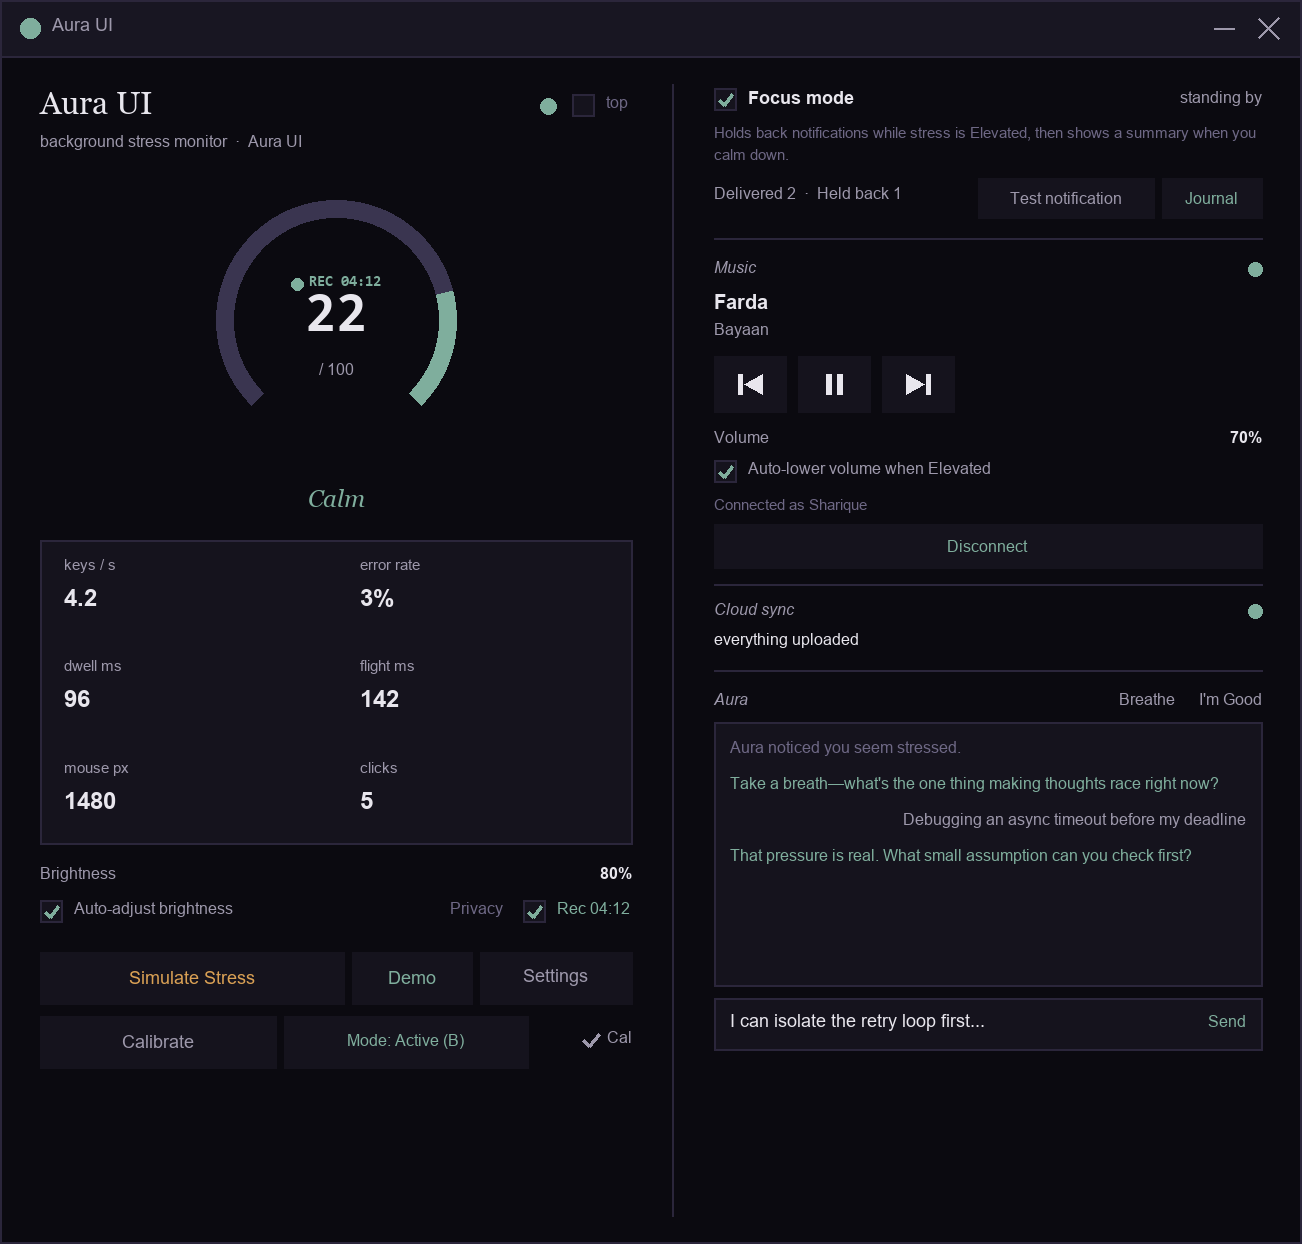
\includegraphics[width=0.92\textwidth,max height=0.50\textheight,keepaspectratio]{docs/figures/ui_main_dashboard.png}
    \caption{\textbf{Aura UI Main Dashboard (Two-Column Layout).} \textit{Left column:} live circular stress dial with active session timer (\texttt{$\bullet$ REC 04:12}), 6-metric behavioral telemetry grid, display brightness status, \uictrl{Privacy} gate, \uictrl{Record session} toggle, \uictrl{Simulate Stress}, \uictrl{Demo}, \uictrl{Settings}, \uictrl{Calibrate}, and study condition button (\uictrl{Mode: Active (B)}). \textit{Right column:} Focus notification gatekeeper, Spotify playback \& auto-volume, Firebase cloud sync status, and conversational Aura check-in panel.}
    \label{fig:dashboard}
\end{figure}

\begin{figure}[htbp]
    \centering
    \begin{minipage}[t]{0.31\textwidth}
        \centering
        \includegraphics[width=\linewidth,max height=0.25\textheight,keepaspectratio]{{"mild stress.png"}}
        \caption{\textbf{Tier 1 (Mild, 42/100):} Amber dial; display eases toward 65\% and 5000\,K.}
        \label{fig:mild_ui}
    \end{minipage}
    \hfill
    \begin{minipage}[t]{0.31\textwidth}
        \centering
        \includegraphics[width=\linewidth,max height=0.25\textheight,keepaspectratio]{{"elevated stress.png"}}
        \caption{\textbf{Tier 2 (Elevated, 61/100):} Rose dial; Focus mode blocking alerts at 3500\,K.}
        \label{fig:elev_ui}
    \end{minipage}
    \hfill
    \begin{minipage}[t]{0.31\textwidth}
        \centering
        \includegraphics[width=\linewidth,max height=0.25\textheight,keepaspectratio]{{"breathing screen.png"}}
        \caption{\textbf{Breathing Guide:} Physiological sigh (1.5\,s + 0.5\,s inhale, 6\,s exhale).}
        \label{fig:breath_ui}
    \end{minipage}
\end{figure}

\subsection{Control-by-Control Reference}
\begin{table}[htbp]
\centering
\scriptsize
\begin{tabularx}{\textwidth}{l l X}
\toprule
\textbf{Section} & \textbf{UI Element} & \textbf{Purpose \& Behavior} \\
\midrule
\textbf{Header} & Status dot \& \uictrl{top} & Live tier color dot (\textit{Calm/Mild/Elevated}); ticking \uictrl{top} keeps Aura floating above other windows. Closing the window minimizes it to the Windows system tray. \\
\textbf{Dial \& Stats} & Score dial \& 6 cells & Displays 0--100 smoothed stress score, live \texttt{$\bullet$ REC MM:SS} / \texttt{SIM} badge, and 5\,s rolling \texttt{keys/s}, \texttt{error rate}, \texttt{dwell ms}, \texttt{flight ms}, \texttt{mouse px}, and \texttt{clicks}. \\
\textbf{Display} & \uictrl{Auto-adjust brightness} & Opt-in toggle for smooth screen dimming \& Kelvin warming. Unchecking (or quitting) restores original brightness and 6500\,K gamma automatically. \\
\textbf{Research} & \uictrl{Privacy} \& \uictrl{Record session} & Opens informed consent dialog; ticking \uictrl{Record session} logs telemetry to \texttt{data/sessions/} (redirects to Privacy if consent is not on file). Unchecking auto-opens the Journal to finalize ratings. \\
\textbf{Testing} & \uictrl{Simulate Stress} \& \uictrl{Demo} & \uictrl{Simulate Stress} injects 10\,s of Elevated stress (82/100) and resets intervention cooldowns; \uictrl{Demo} opens the 4-stage presentation controller and manual tier overrides. \\
\textbf{Tuning} & \uictrl{Settings} \& \uictrl{Calibrate} & Adjusts weights, smoothing, decay speed, and per-tier brightness/Kelvin/volume targets; \uictrl{Calibrate} launches the 30-second resting baseline modal (\uictrl{$\checkmark$ Cal} badge). \\
\textbf{Study Arm} & \uictrl{Mode: Active (B) / Control (A)} & One-click experimental condition switch. \textbf{Control (A)} logs telemetry silently with all visual, DND, audio, breathing, and chat interventions suppressed. \\
\textbf{Focus Mode} & \uictrl{Focus mode}, \uictrl{Test notification} & Suppresses alerts when \textit{Elevated} (unless Control A); shows amber summary digest toast once Calm returns; \uictrl{Journal} opens reflection \& past sessions. \\
\textbf{Music} & Playback \& \uictrl{Connect Spotify} & Links your Spotify account via browser PKCE; optionally ducks volume by tier when \uictrl{Auto-lower volume when Elevated} is checked. \\
\textbf{Cloud Sync} & Status indicator & Shows \texttt{everything uploaded} (green), queued count (amber), or retry error (red); retries every 5\,min in background. \\
\textbf{Aura Chat} & \uictrl{Breathe}, \uictrl{I'm Good}, input & Opens on-demand breathwork or dismisses chat (resetting 5-min check-in timer); type any message and press Enter to talk to Aura anytime. \\
\bottomrule
\end{tabularx}
\caption{Complete reference of controls across both columns of Aura UI.}
\label{tab:controls}
\end{table}

% ============================================================================
\section{Privacy, Calibration \& Journal Workflows}
% ============================================================================

Before collecting any human session data, Aura UI guides the participant through three purpose-built modal dialogs so research ethics, baseline personalization, and ground-truth labels remain transparent and effortless.

\begin{figure}[htbp]
    \centering
    \begin{minipage}[t]{0.48\textwidth}
        \centering
        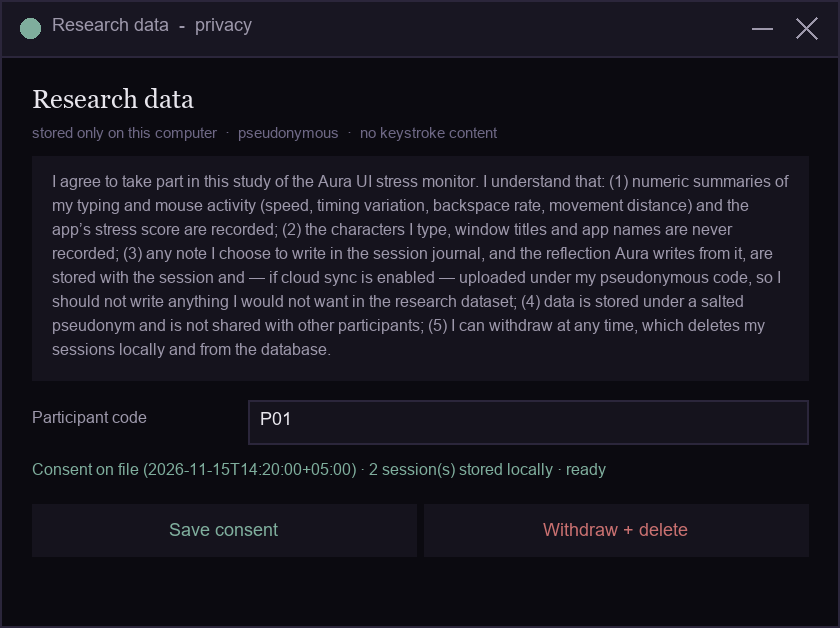
\includegraphics[width=\linewidth,max height=0.29\textheight,keepaspectratio]{docs/figures/ui_privacy_consent.png}
        \caption{\textbf{Research Consent Gate (\uictrl{Privacy}):} Recording is disabled until consent is explicitly saved under a participant code (e.g., \texttt{P01}). Clicking \uictrl{Withdraw + delete} erases both local JSONL files and uploaded Firestore documents.}
        \label{fig:consent}
    \end{minipage}
    \hfill
    \begin{minipage}[t]{0.48\textwidth}
        \centering
        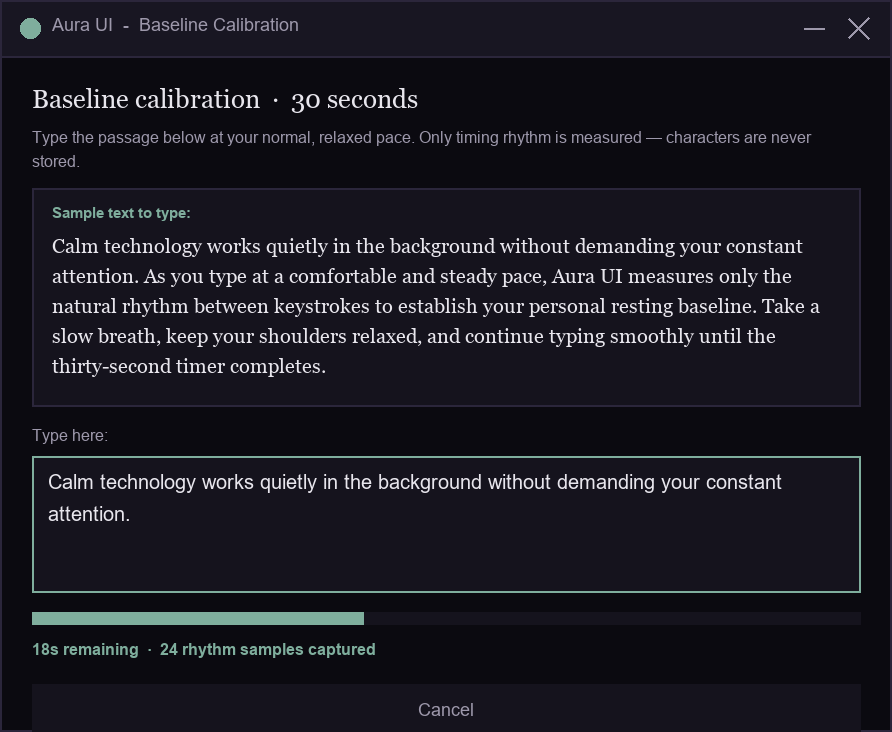
\includegraphics[width=\linewidth,max height=0.29\textheight,keepaspectratio]{docs/figures/ui_calibration_modal.png}
        \caption{\textbf{30-Second Baseline Calibration (\uictrl{Calibrate}):} Auto-focused prose typing task measuring personal resting keystroke CoV and error rate without storing characters.}
        \label{fig:calibration}
    \end{minipage}
\end{figure}

\begin{figure}[htbp]
    \centering
    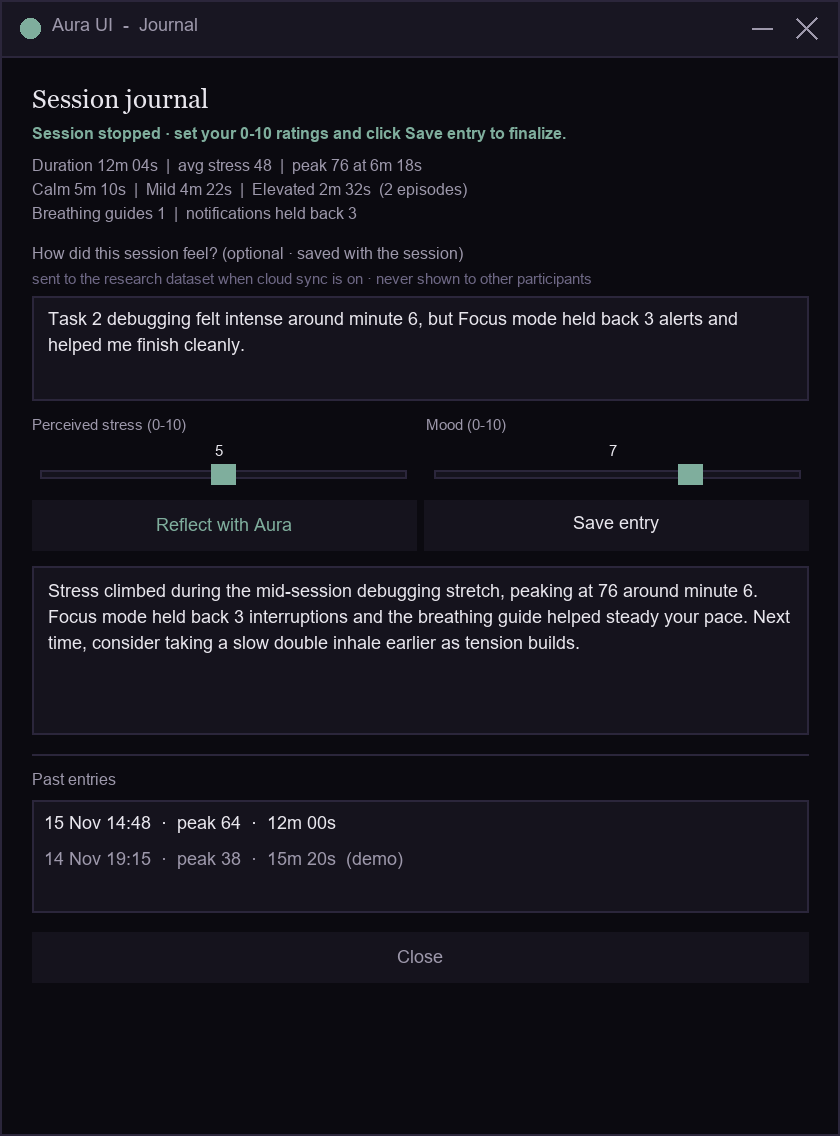
\includegraphics[width=0.56\textwidth,max height=0.40\textheight,keepaspectratio]{docs/figures/ui_session_journal.png}
    \caption{\textbf{Post-Session Journal (\uictrl{Journal}):} Unchecking \uictrl{Record session} opens this dialog automatically in finalize mode so the participant sets \textbf{Perceived stress (0--10)} and \textbf{Mood (0--10)}, optionally requests an AI reflection (\uictrl{Reflect with Aura}), and clicks \uictrl{Save entry} to close and queue the hash-chained session.}
    \label{fig:journal}
\end{figure}

% ============================================================================
\section{Installation, Configuration \& Standalone Build}
% ============================================================================

\subsection{Option A: Running from Source (Developers \& Lab Hosts)}
Requires \textbf{Python 3.9+} on Windows 10/11 (recommended for native WMI/DDC brightness, Windows GDI color temperature, and Windows Focus Assist DND):
\begin{verbatim}
git clone https://github.com/ShariqueBaig/HCI-project.git
cd HCI-project
pip install -r requirements.txt
pip install matplotlib             # optional: required for plot_session.py
python run.py
\end{verbatim}
You can also install Aura UI as a CLI command via \texttt{pyproject.toml}:
\begin{verbatim}
pip install -e ".[plots]"
aura-ui
\end{verbatim}

\subsection{Option B: Building \& Shipping Zero-Setup \texttt{AuraUI.exe} (Field Testing)}
To distribute Aura UI to participants' laptops with \textbf{zero Python installation and zero config steps}:
\begin{verbatim}
pip install ".[build]"
python -m PyInstaller --onefile --noconsole --name "AuraUI" ^
    --add-data "aura_defaults.json;." run.py
\end{verbatim}
This produces a single \texttt{dist/AuraUI.exe} binary. \texttt{aura\_defaults.json} bundles public identifiers (Firebase project ID + Web API key + Spotify PKCE Client ID) so anonymous cloud sync works out of the box. Note that participants should place \texttt{AuraUI.exe} in a writable folder such as \texttt{Desktop} or \texttt{Documents} (not \texttt{Program Files}), and click \textit{More info $\rightarrow$ Run anyway} if Windows SmartScreen prompts on first launch.

\subsection{Optional Secrets (\texttt{secrets.json} \& \texttt{firebase\_config.json})}
\begin{itemize}[leftmargin=1.5em, itemsep=2pt]
    \item \textbf{Aura Cloud LLM (OpenRouter):} Copy \texttt{secrets.example.json} to \texttt{secrets.json} and add \texttt{"openrouter\_api\_key": "sk-or-..."} (or set \texttt{OPENROUTER\_API\_KEY}). The controller tries four free OpenRouter models in sequence (\texttt{nvidia/nemotron-3-super-120b-a12b:free}, \texttt{meta-llama/llama-3.3-70b-instruct:free}, \texttt{google/gemma-3-27b-it:free}, \texttt{openrouter/free}) and falls back seamlessly to its built-in empathetic local coach if offline or if no key is provided.
    \item \textbf{Spotify:} In the app, click \uictrl{Connect Spotify} under Music and sign in via browser PKCE (redirect URI \texttt{http://127.0.0.1:8080}).
    \item \textbf{Firebase Firestore Sync:} Already enabled via \texttt{aura\_defaults.json} (or override with \texttt{firebase\_config.json}; see \texttt{FIREBASE\_SETUP.md}). Verify anytime with \texttt{python -m backend.firebase\_sync --check}.
\end{itemize}

% ============================================================================
\section{Quick 2-Minute Evaluator Walkthrough}
% ============================================================================

Anyone testing Aura UI for the first time can observe every feature working end-to-end in under two minutes:
\begin{enumerate}[leftmargin=1.5em, itemsep=3pt]
    \item \textbf{Live Sensing Baseline (20\,s):} Launch \texttt{python run.py} (ensure \uictrl{Mode: Active (B)} is shown) and type normally in any editor. Watch \texttt{keys/s}, \texttt{dwell ms}, \texttt{flight ms}, and \texttt{mouse px} update every 333\,ms while the score stays in \textcolor{AuraTeal}{Calm} (0--29). Tick \uictrl{Auto-adjust brightness} to let display modulation run.
    \item \textbf{Test Focus Mode in Calm (10\,s):} Click \uictrl{Test notification} on the right panel. A green \textit{Delivered} toast appears immediately in the bottom-right corner.
    \item \textbf{Trigger Stress \& Ambient Interventions (15\,s):} Click \uictrl{Simulate Stress} (or click \uictrl{Demo} $\rightarrow$ \uictrl{Run full scripted demo}). Within seconds:
    \begin{itemize}[leftmargin=1.2em, itemsep=1pt]
        \item Dial climbs into \textcolor{AuraRose}{Elevated} ($>60$); display dims and warms toward 3500\,K.
        \item Focus status turns red (\texttt{BLOCKING notifications}). Clicking \uictrl{Test notification} now shows a red \textit{Held back by Focus mode} card and increments \texttt{Held back}.
        \item After 3 seconds in Elevated, the physiological sighing popup (\textbf{Breathe}) opens and \textbf{Aura Chat} initiates a proactive empathetic check-in. Reply in the chat box, or click \uictrl{I'm Good} once ready.
    \end{itemize}
    \item \textbf{Observe Recovery Digest (5\,s):} Wait $\approx 3$ seconds after simulation stops; stress decays smoothly back to \textcolor{AuraTeal}{Calm}, screen brightness/warmth restores, and Focus mode delivers an amber summary toast listing all held apps.
    \item \textbf{Try Calibration \& Journal (30\,s):} Click \uictrl{Privacy} $\rightarrow$ enter code \texttt{TEST} $\rightarrow$ \uictrl{Save consent}; click \uictrl{Calibrate} and type the passage; tick and uncheck \uictrl{Record session} to inspect the finalized \textbf{Journal} modal.
\end{enumerate}

% ============================================================================
\section{Human-Subjects Pilot Testing Protocol (35 Min, $N = 8$--$12$)}
% ============================================================================

To evaluate construct validity ($H_4$), workload reduction ($H_1$), recovery speed ($H_2$), and system usability ($H_3$), run a counterbalanced within-subjects ($A/B$) study comparing \textbf{Condition A (Control: \uictrl{Mode: Control (A)})} against \textbf{Condition B (Intervention: \uictrl{Mode: Active (B)})} across two equivalent 12-minute cognitive stressor tasks (e.g., timed debugging + timed analytical writing).

\begin{table}[htbp]
\centering
\small
\begin{tabularx}{\textwidth}{l l c l c l}
\toprule
\textbf{Participant} & \textbf{Session 1 Code} & \textbf{Condition} & \textbf{Task} & \textbf{Session 2 Code} & \textbf{Condition / Task} \\
\midrule
P01, P05, P09 & \texttt{P01-A}, \dots & Control (A) & Task 1 & \texttt{P01-B}, \dots & Active (B) / Task 2 \\
P02, P06, P10 & \texttt{P02-B}, \dots & Active (B) & Task 1 & \texttt{P02-A}, \dots & Control (A) / Task 2 \\
P03, P07, P11 & \texttt{P03-A}, \dots & Control (A) & Task 2 & \texttt{P03-B}, \dots & Active (B) / Task 1 \\
P04, P08, P12 & \texttt{P04-B}, \dots & Active (B) & Task 2 & \texttt{P04-A}, \dots & Control (A) / Task 1 \\
\bottomrule
\end{tabularx}
\caption{Counterbalancing matrix eliminating order and task-difficulty bias across $N=8$--$12$ participants.}
\label{tab:counterbalance}
\end{table}

\begin{enumerate}[leftmargin=1.5em, itemsep=2pt]
    \item \textbf{Phase 1 --- Consent \& 30\,s Calibration (3\,min):} Open \uictrl{Privacy} $\rightarrow$ save participant code \& consent; click \uictrl{Calibrate} and type comfortably for 30\,s to personalize resting CoV and error baselines.
    \item \textbf{Phase 2 --- Session 1 (12\,min):} Set the Mode toggle to Condition A or B, tick \uictrl{Record session} (\texttt{$\bullet$ Rec 00:00}), run Task 1, and click \uictrl{Test notification} at \textbf{3:00}, \textbf{6:00}, and \textbf{9:00}.
    \item \textbf{Phase 3 --- Mid-Study Assessment (3\,min):} Uncheck \uictrl{Record session} at \textbf{12:00}; complete the auto-opened Journal sliders (\textit{Perceived stress} and \textit{Mood} 0--10) and click \uictrl{Save entry}; administer NASA-TLX \#1.
    \item \textbf{Phase 4 --- Session 2 (12\,min):} Toggle Mode to the opposite condition, tick \uictrl{Record session}, run Task 2 with alerts at \textbf{3:00}, \textbf{6:00}, and \textbf{9:00}.
    \item \textbf{Phase 5 --- Post-Study Assessment (5\,min):} Uncheck \uictrl{Record session} $\rightarrow$ save Journal ratings $\rightarrow$ administer NASA-TLX \#2, 10-item SUS questionnaire, and 3-question semi-structured debrief.
\end{enumerate}

\notebox{Control vs.\ Active Guardrail}{When \uictrl{Mode: Control (A)} is selected, Aura UI automatically disables brightness/Kelvin shifts, Windows Focus Assist, breathing popups, music auto-volume, and proactive check-ins, and records \texttt{condition="control"} in \texttt{sessions.csv} even if the checkboxes remain checked.}

% ============================================================================
\section{Instrument Validation \& Data Analysis Playbook}
% ============================================================================

Prior to human testing, the scoring instrument was benchmarked over 1,200 ticks (400\,s balanced protocol across REST, CALM, MILD, and ELEV blocks, \texttt{experiments/run\_experiment.py}):
\begin{itemize}[leftmargin=1.5em, itemsep=2pt]
    \item \textbf{Three-Class Accuracy:} \textbf{93.3\%} overall (1,120 / 1,200 ticks), with 91.3\%--95.3\% accuracy per regime.
    \item \textbf{ROC Discrimination:} \textbf{AUC = 0.994}; deployed threshold ($\ge 60$) achieves \textbf{95.0\% recall} at just \textbf{1.2\% false-positive rate}.
    \item \textbf{Latency \& Recovery:} \textbf{1.00\,s} mean detection latency into Elevated; \textbf{2.00\,s} recovery back to Calm via proportional release + hysteresis.
    \item \textbf{Cryptographic Audit:} 1,202 / 1,202 records hash-verified; strict whitelist proved typed characters and window titles are dropped before disk.
\end{itemize}

\begin{figure}[htbp]
    \centering
    \begin{minipage}[t]{0.32\textwidth}
        \centering
        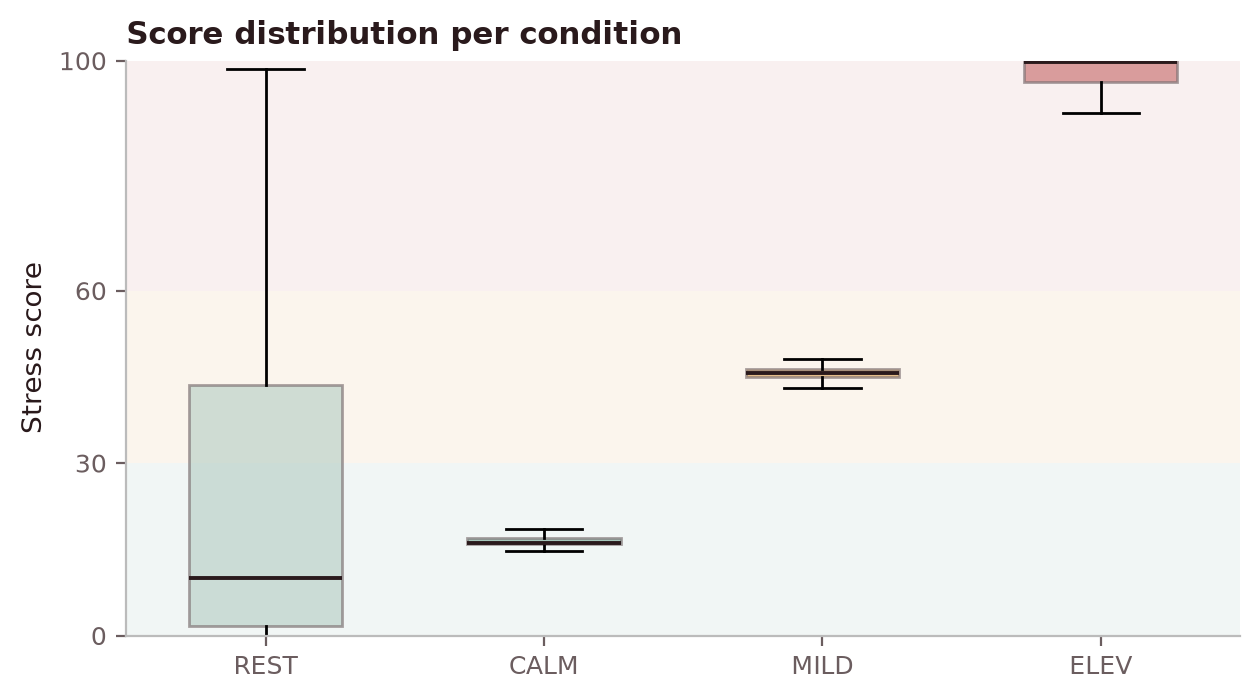
\includegraphics[width=\linewidth,max height=0.22\textheight,keepaspectratio]{Phase_2_Submission/figures/f2_score_by_condition.png}
        \caption{\textbf{Score Distribution:} Clean separation across REST, CALM, MILD, and ELEV regimes.}
        \label{fig:val_dist}
    \end{minipage}
    \hfill
    \begin{minipage}[t]{0.32\textwidth}
        \centering
        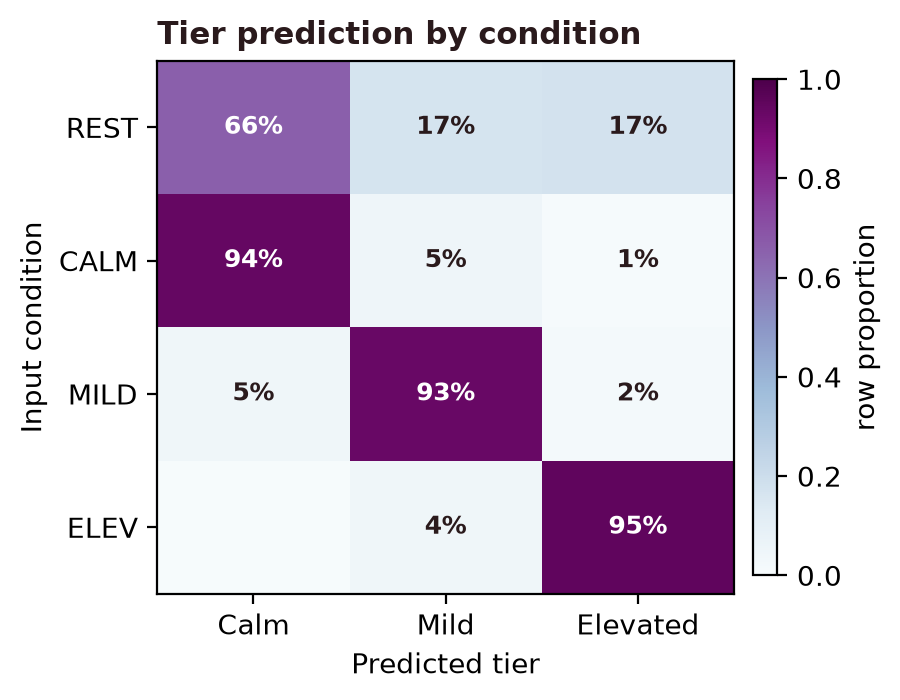
\includegraphics[width=\linewidth,max height=0.22\textheight,keepaspectratio]{Phase_2_Submission/figures/f3_confusion.png}
        \caption{\textbf{Tier Confusion Matrix:} 91.3\%--95.3\% class alignment across all four states.}
        \label{fig:val_conf}
    \end{minipage}
    \hfill
    \begin{minipage}[t]{0.32\textwidth}
        \centering
        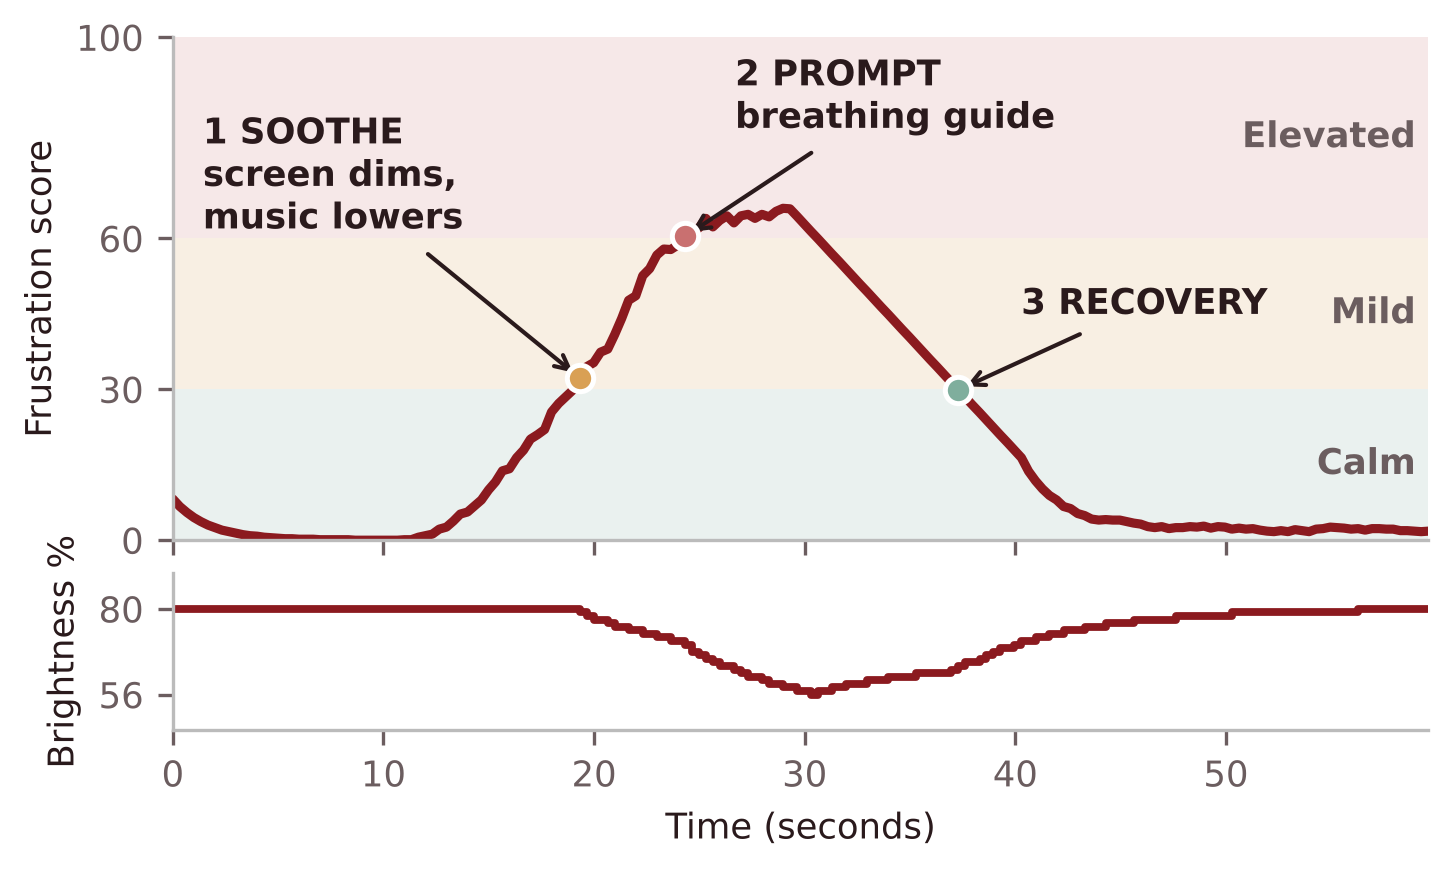
\includegraphics[width=\linewidth,max height=0.22\textheight,keepaspectratio]{aura_session_chart_poster.png}
        \caption{\textbf{Live Recovery Curve:} Soothe dimming, breathing prompt, and Calm recovery.}
        \label{fig:val_live}
    \end{minipage}
\end{figure}

\subsection{Post-Study Export, Audit \& Plotting Commands}
After running pilot sessions, verify cryptographic integrity, export de-identified CSVs, and render timeline plots with three commands:
\begin{verbatim}
# 1. Verify tamper-evident SHA-256 hash chains across all sessions
python -c "from backend import research; import json; print(json.dumps(research.audit(), indent=2))"

# 2. Export de-identified summary (sessions.csv) and 3 Hz tick rows (ticks.csv)
python -c "from backend import research; print(research.export_dataset('human_pilot_export'))"

# 3. Generate publication-ready PNGs from the newest .jsonl session (or pass path)
python plot_session.py [optional/path/to/session.jsonl] [--start 0 --end 720]
\end{verbatim}

\notebox{Troubleshooting Tip}{If \texttt{research.audit()} returns an empty session list after field testing on multiple laptops, check the Cloud Sync status in Aura UI (\texttt{everything uploaded}) and inspect the \texttt{aura\_sessions} collection in the Firebase Console; if running offline, copy the participant's \texttt{data/sessions/} folder into the local workspace before calling \texttt{export\_dataset()}.}

\end{document}
